\documentclass[captions=tableheading]{scrartcl}

\usepackage{amsmath}
\usepackage{amssymb}
\usepackage[utf8]{inputenc}
\usepackage[T1]{fontenc}
\usepackage{lmodern}
\usepackage{ngerman}
\usepackage{geometry}
\usepackage{graphicx}
\usepackage{wrapfig}
\usepackage{caption}
\usepackage{wasysym}
\usepackage[separate-uncertainty=true]{siunitx}
\usepackage{picinpar}
\usepackage{tikz}
\usepackage{float}
\usepackage{booktabs}

\renewcommand{\figurename}{Abb.}
\usepackage[
	colorlinks=true,
	urlcolor=blue,
	linkcolor=black
]{hyperref}


%Hier Titel und so
\newcommand{\versuchnummer}{V60} 
\newcommand{\versuchname}{Der Diodenlaser} 
\newcommand{\versuchdatum}{23.01.2017} 


\title{Versuch \versuchnummer\\ \versuchname}
\subtitle{Physikalisches Fortgeschrittenenpraktikum}
\author{Robert Rauter und Björn Lindhauer}
\date{\versuchdatum} 
\begin{document}
\begin{titlepage}
{\large \versuchdatum}
\vspace{7cm}
\begin{center}
\textbf{\huge Versuch \versuchnummer}\\\vspace{0.5cm}
\textbf{\huge \versuchname}\\
\vspace{0.2cm}
\textbf{Physikalisches Fortgeschrittenenpraktikum}\\
\vspace{9cm}

{\Large Robert Rauter \ \ \hspace{1.5cm} und \hspace{1.5cm} Björn Lindhauer}\\
{ \url{robert.rauter@tu-dortmund.de} \ \ \hspace{2cm} \url{bjoern.lindhauer@tu-dortmund.de}}
\end{center}
\end{titlepage}
\section{Einleitung}

\section{Theoretische Grundlagen}

\section{Aufbau}

\section{Durchführung}

\subsection{Justierung des Strahlengangs}

\begin{center}
	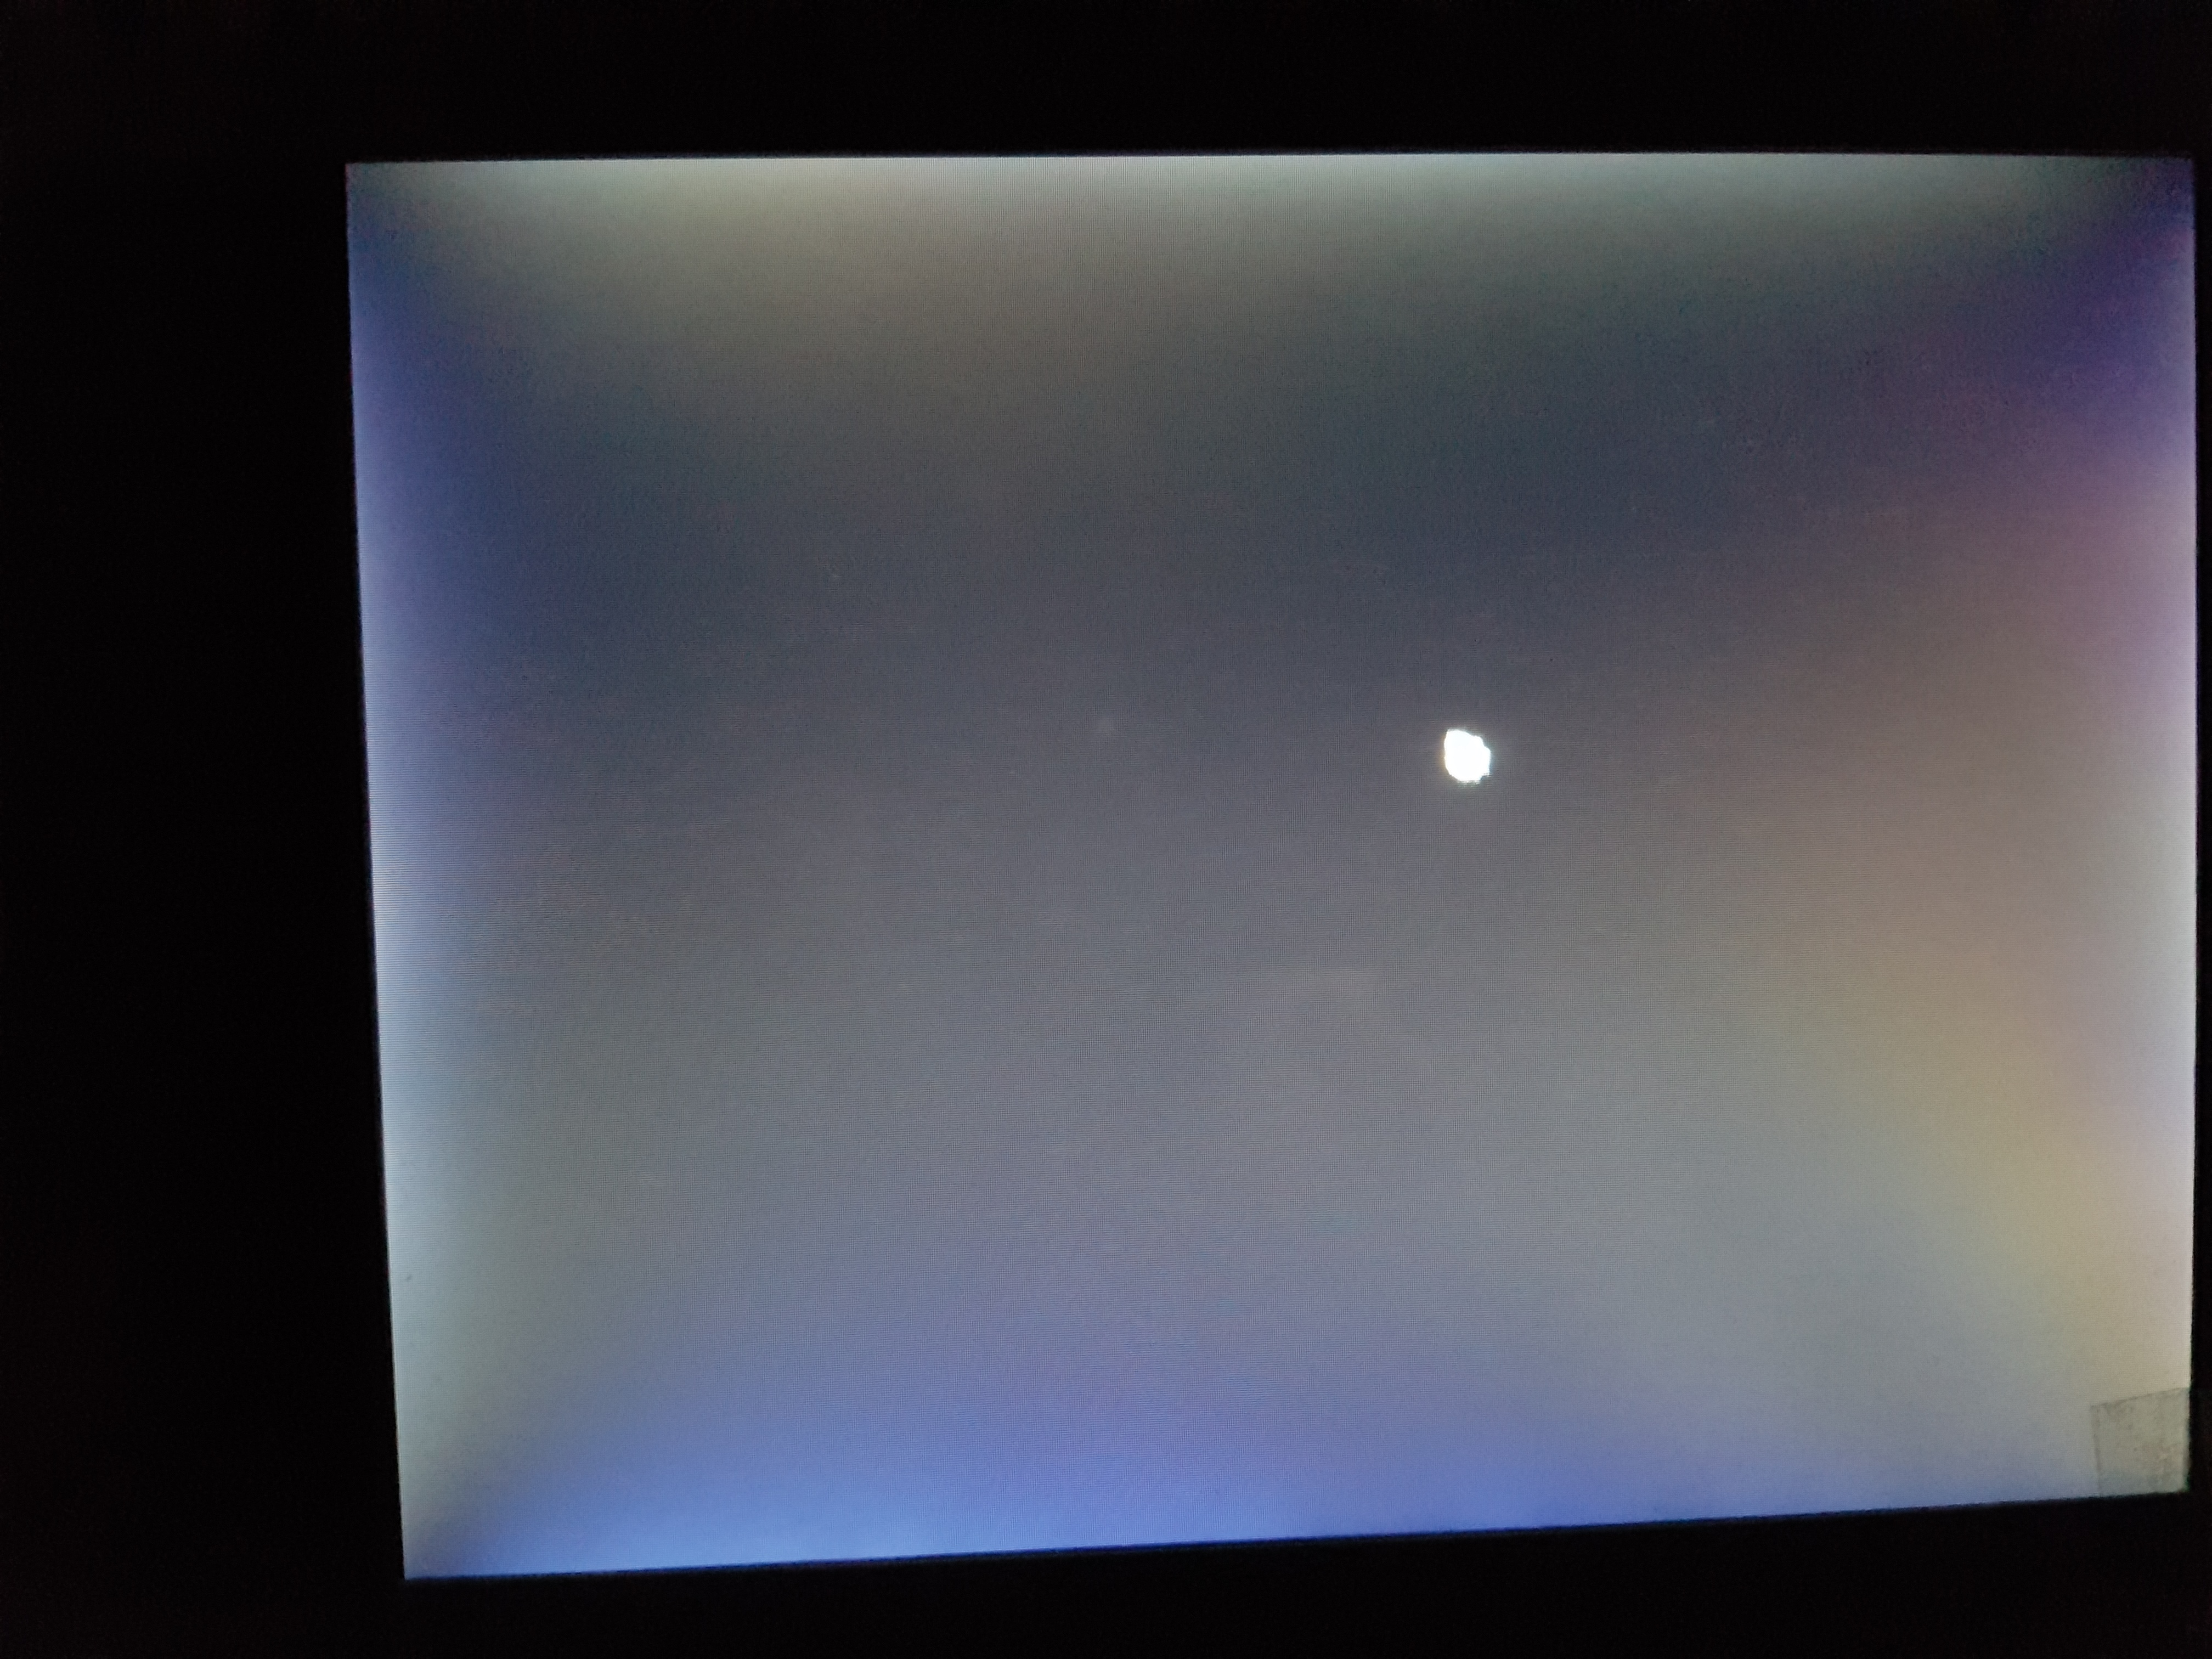
\includegraphics[width=10cm]{images/led_spot.jpg}
	\captionof{figure}{Beobachtetes Ausgangssignal des Diodenlasers unterhalb der Grenzstromstärke}
	\label{fig:led}
\end{center}

\begin{center}
	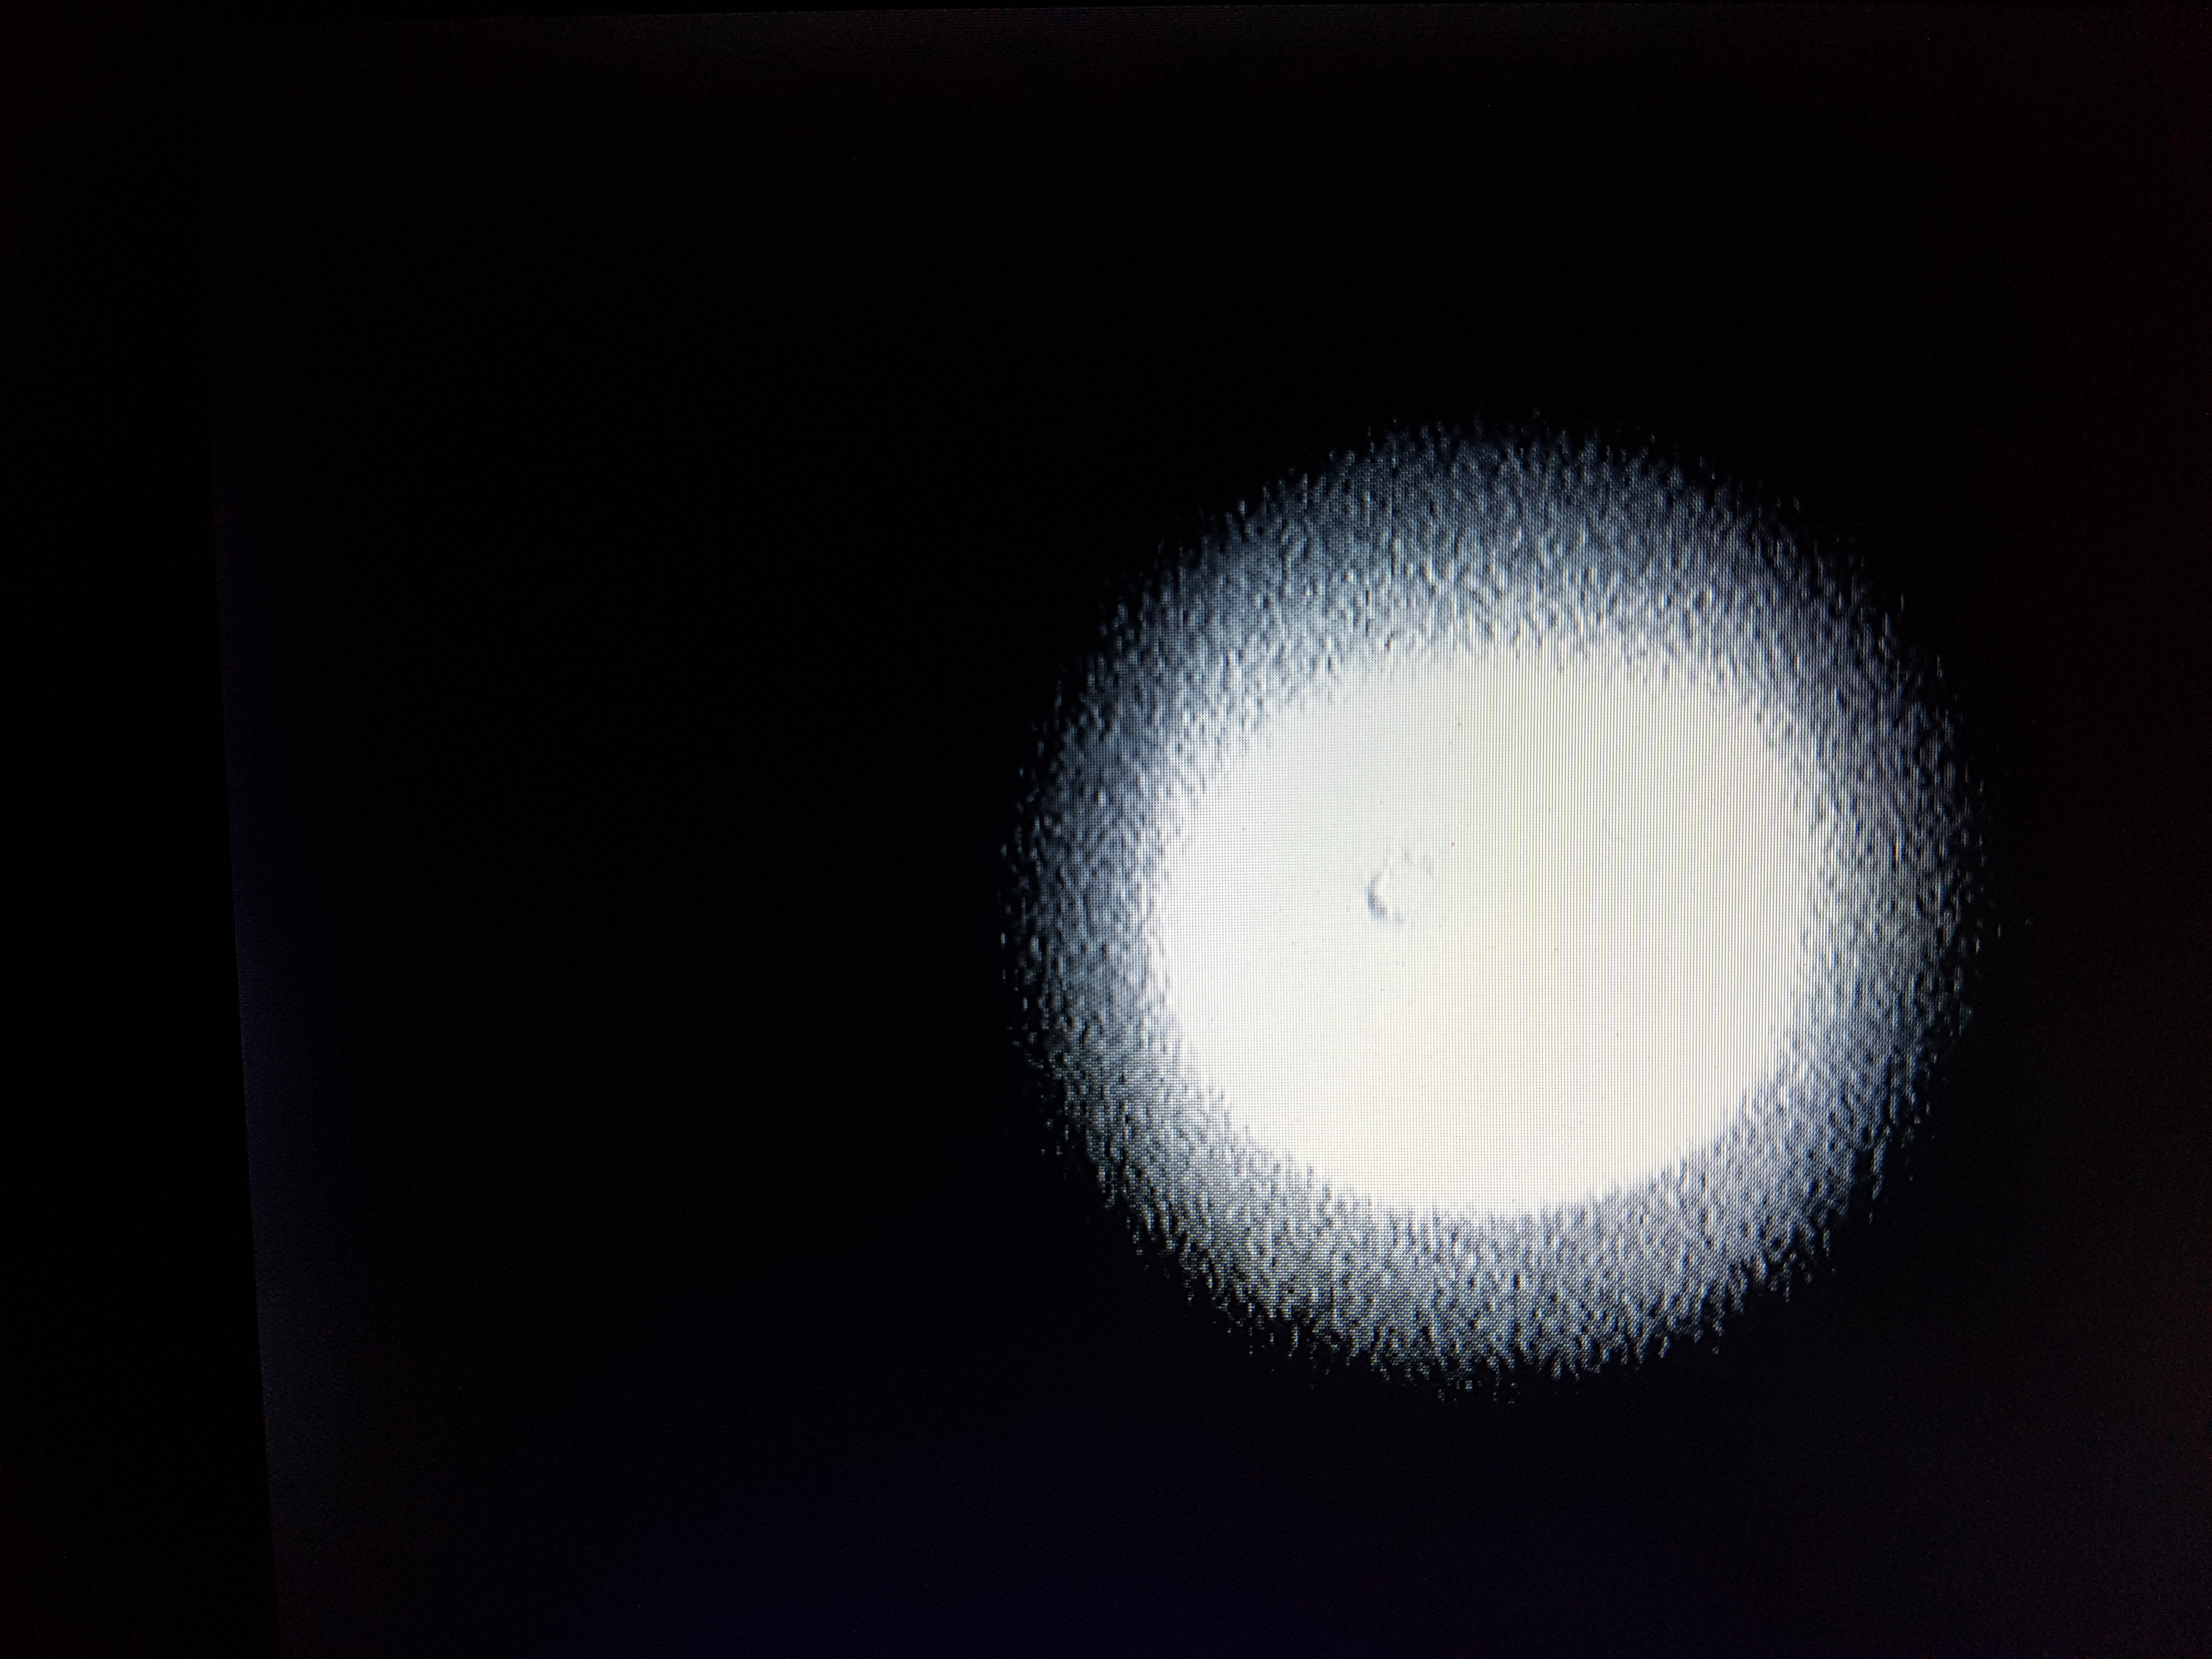
\includegraphics[width=10cm]{images/over_threshold.jpg}
	\captionof{figure}{Beobachtetes Ausgangssignal des Diodenlaser oberhalb der Grenzstromstärke}
	\label{fig:over_threshold}
\end{center}

\subsection{Beobachtung der Rubidium-Resonanz}

\begin{center}
	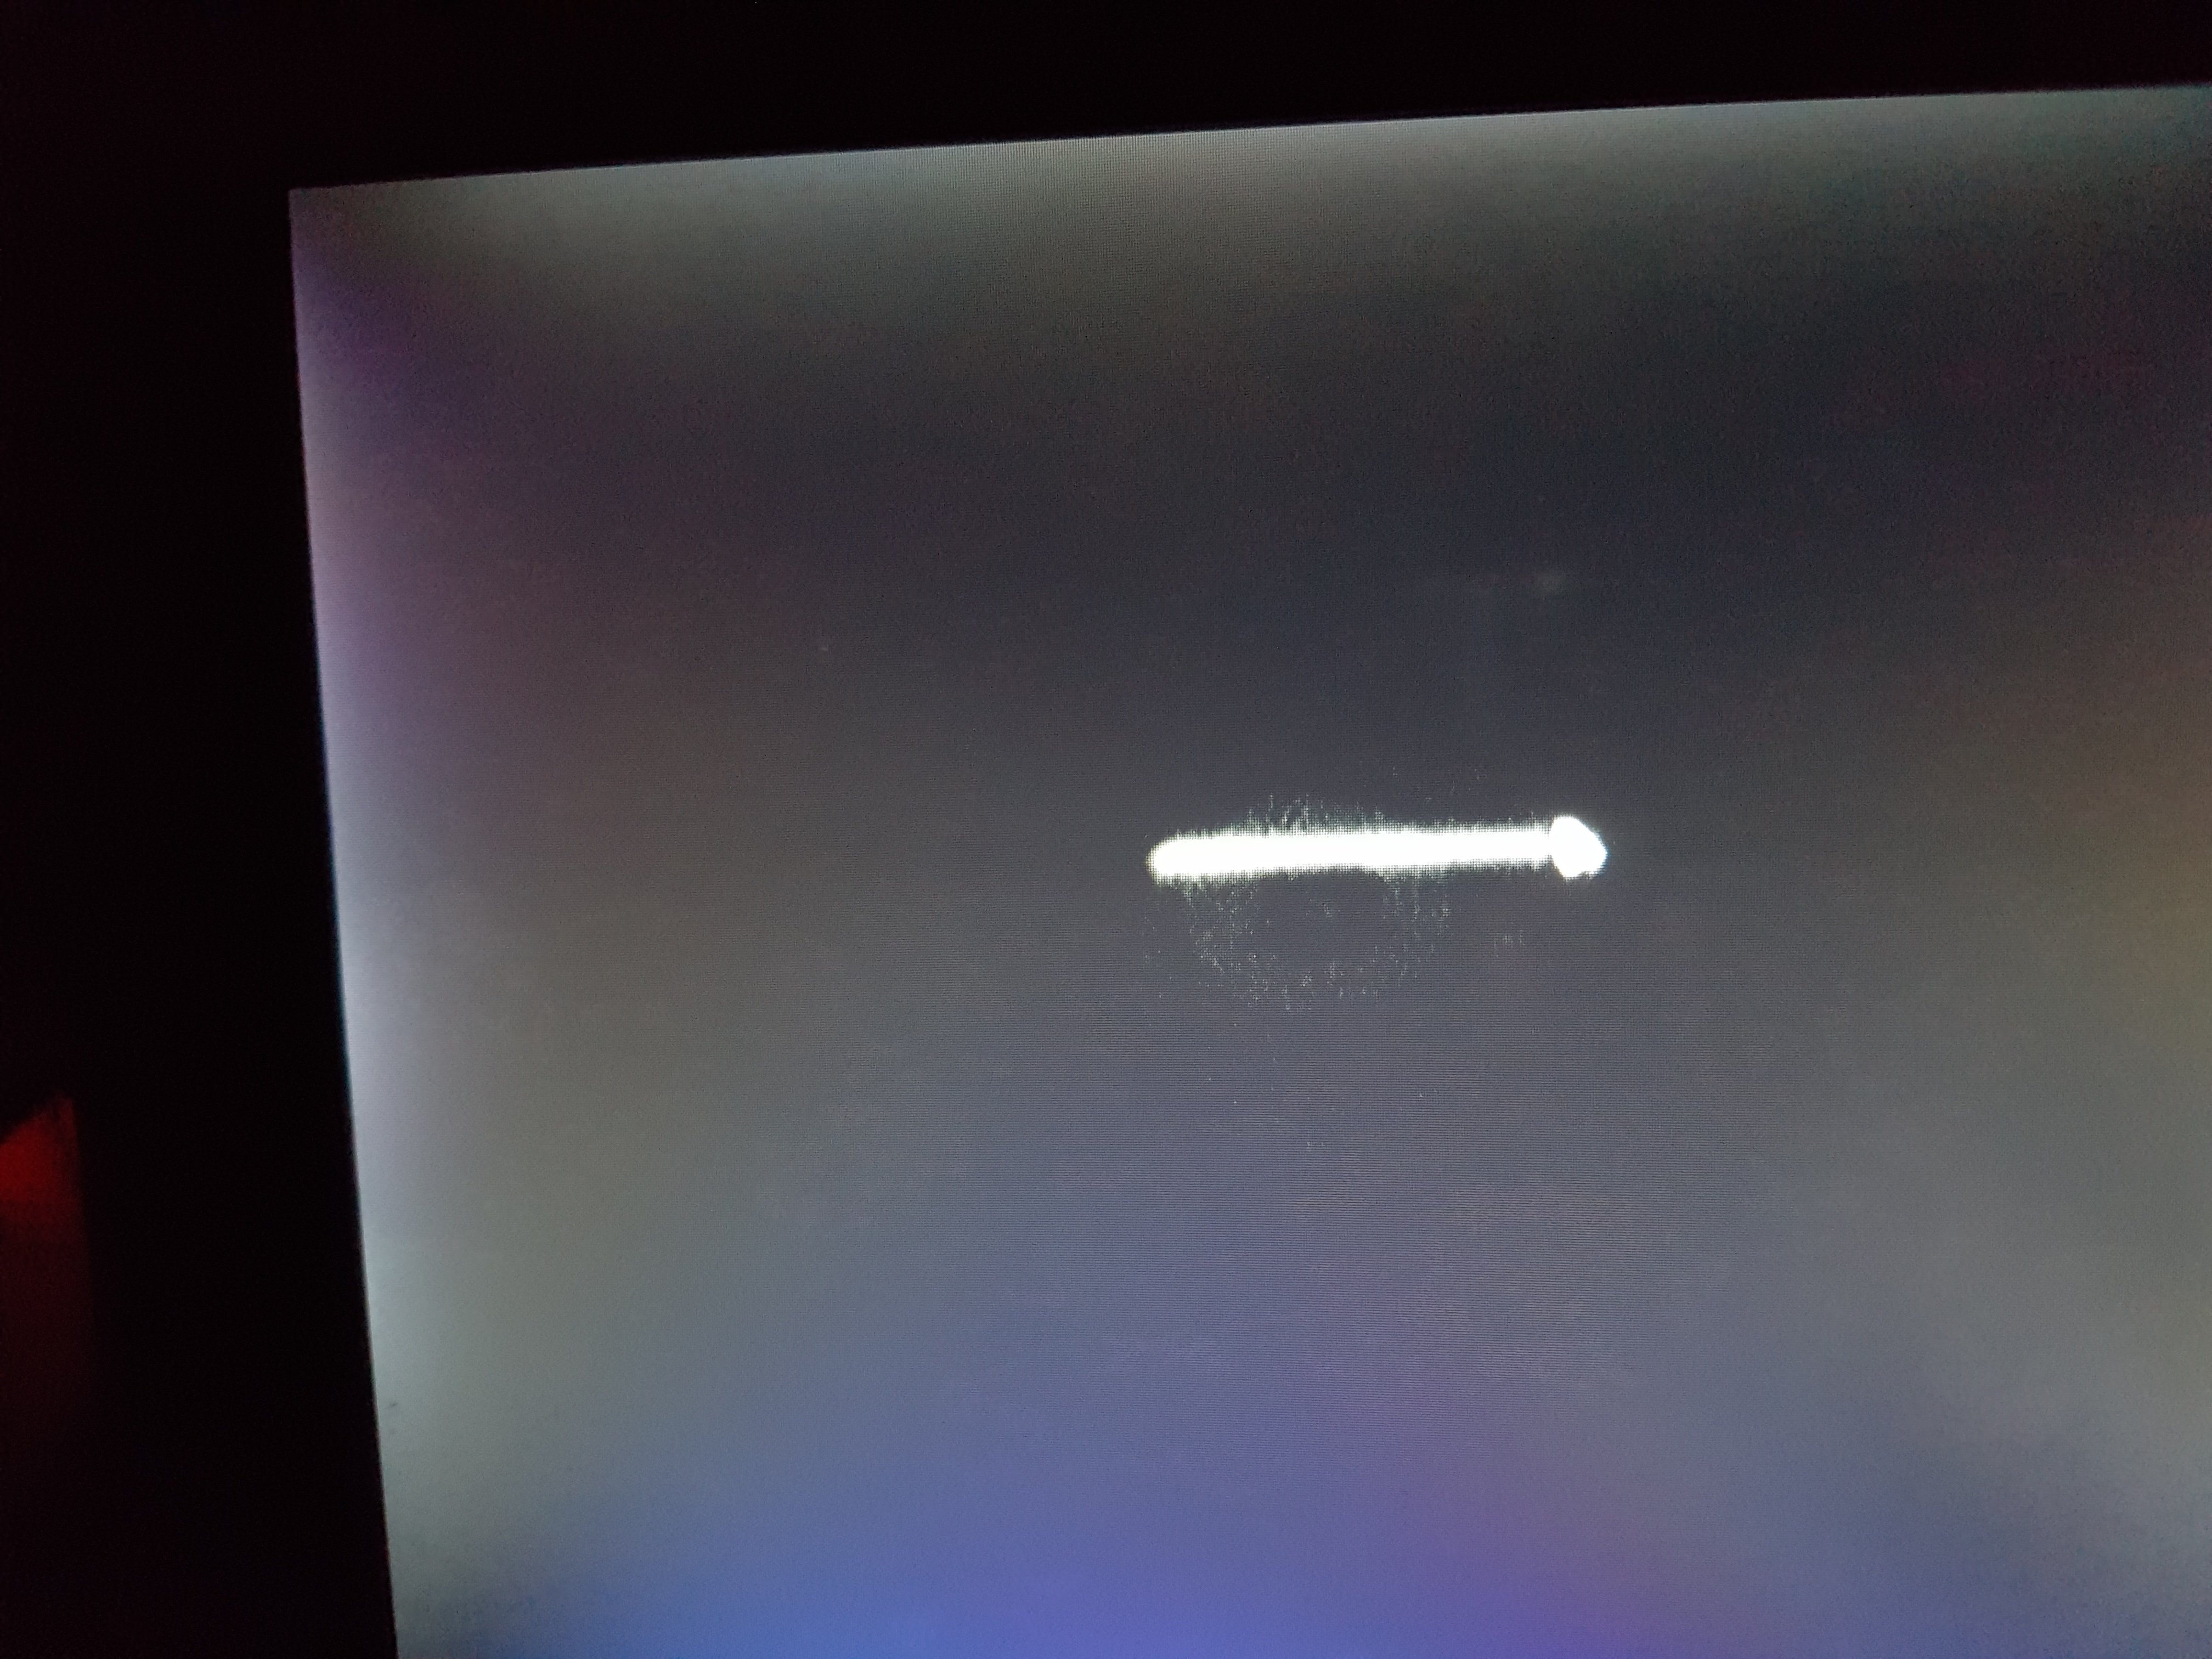
\includegraphics[width=10cm]{images/resonanz_bild.jpg}
	\captionof{figure}{Mit Kamera detektiertes Resonanzsignal}
	\label{fig:resonanzbild}
\end{center}

\begin{center}
	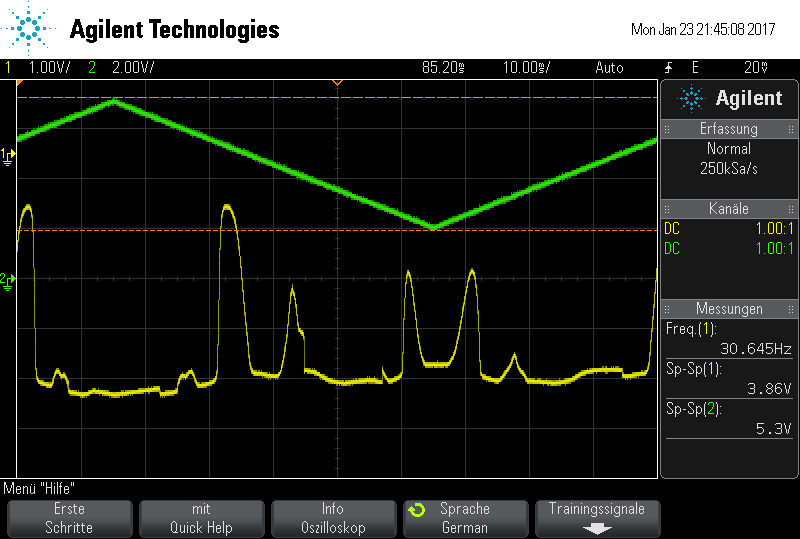
\includegraphics[width=10cm]{images/scope_22.png}
	\captionof{figure}{Resonanzspektrum vin Rubidium}
	\label{fig:resonanz}
\end{center}

\subsection{Bereinigung des Resonanzsignals}

\begin{center}
	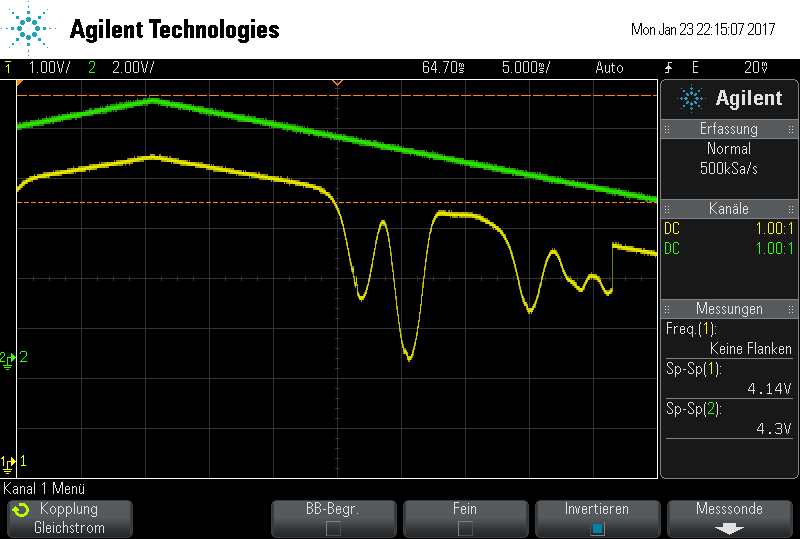
\includegraphics[width=10cm]{images/resonanz.png}
	\captionof{figure}{Resonanzlinien der Rubidium-Probe, mit Hintergrund-Intensität}
	\label{fig:resonanzlinien}
\end{center}

\begin{center}
	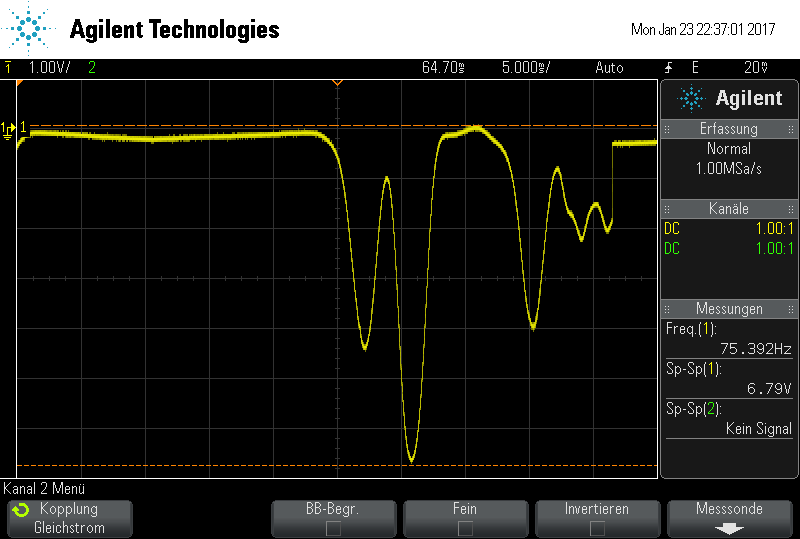
\includegraphics[width=10cm]{images/resonanz_bereinigt.png}
	\captionof{figure}{Um Hintergrund bereinigte Resonanzlinien der Rubidium-Probe}
	\label{fig:resonanzlinien_mh}
	\end{center}

\section{Diskussion}

\section{Quellen}
{[1]} Physikalisches Praktikum, TU Dortmund: \\
\textit{Versuchsanleitung zu Versuch 60: Der Diodenlaser} \\
http://129.217.
224.2/HOMEPAGE/PHYSIKER/MASTER/SKRIPT/V60.pdf (letzte Version vom 24.01.2017, 16:00)\\

\end{document}